\section{Related Works}

GeoLifeCLEF 2023 had seven submissions along with baseline results from the organizers \cite{geolifeclef2023}. 
Participants focused on bioclimatic rasters and satellite imagery, leveraging Convolutional Neural Networks (CNN) like ResNets \cite{he2016deep} for feature extraction. 
Participants combined rasters and trained separate models for prediction \cite{Ung2023LeverageSW}. 
Spatial coordinates (longitude/latitude) were commonly used with models like K-Nearest Neighbors (kNN) and Random Forest, yielding surprisingly good results. 
However, the combination of diverse modalities provided in the dataset was rare, with only one participant utilizing time-series data with a 1D Convolutional Network.
% In contrast, our original research plans aims to explore alternative feature extraction methods, such as Tile2Vec for spatial data and Discrete Cosine Transform (DCT) for time series. 
% By adopting these unsupervised techniques, we plan to combine various modalities for prediction, which sets our approach apart from the majority of the participants in GeoLifeClef2023. 
% This multi-modal strategy, we believe, has the potential to enhance prediction accuracy by leveraging the diverse data available in the GeoLifeClef dataset.

\section{Overview}

\begin{figure}[h]
\centering
  \begin{minipage}{0.49\linewidth}
    \begin{lstlisting}[frame=single]

{
  "type": "Polygon",
  "coordinates": [
      [
          [-32.26344, 26.63842],
          [-32.26344, 72.18392],
          [ 35.58677, 72.18392],
          [ 35.58677, 26.63842],
          [-32.26344, 26.63842],
      ]
  ],
}

    \end{lstlisting}
    \caption{GeoJSON polygon definition.}
    \label{lst:geojson-definition}
  \end{minipage}
  \hfill
  \begin{minipage}{0.49\linewidth}
      \centering
      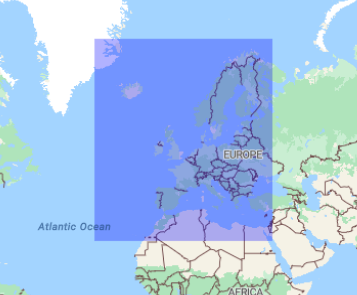
\includegraphics[width=1\linewidth]{figures/geojson.png}
      \caption{Polygon region overlayed on a map.}
      \label{fig:geojson-region}
  \end{minipage}
\end{figure}


The competition has three main components to the dataset. 
The first are the metadata associated with the competition comprising a presence-only training, presence-absence training, and presence-absence test set. 
The metadata provides a mapping between location and the species labels available for supervised training. 
The second are the remote-sensing and raster data provided in pixel format. 
The final component is time series data containing quarterly environmental data over a 20 year period. 

The presence-only training dataset comprises 5,079,797 examples over 3,845,533 survey sites distributed throughout Western Europe.
The dataset is drawn from crowd-sourced data with potential gaps in the reported species.
The presence-absent dataset has stricter semantics -- species not included in the survey are presumed absent.
The training set has 1,483,637 examples over 88,987 sites, while the test set has 4,716 sites.
The datasets include an identifier for the survey site along with latitude and longitude, according to the schema in Listing \ref{lst:schema}.
We compute a projection into EPSG 3035, which allows for Euclidean distance between sites in units of meters. 

\begin{figure}[b]
\begin{lstlisting}[caption={
  Metadata schema for the competition.
}, captionpos=b,label={lst:schema},frame=single]
  |-- dataset: string (nullable = true)
  |-- surveyId: integer (nullable = true)
  |-- lat_proj: double (nullable = true)
  |-- lon_proj: double (nullable = true)
  |-- lat: double (nullable = true)
  |-- lon: double (nullable = true)
  |-- year: integer (nullable = true)
  |-- geoUncertaintyInM: double (nullable = true)
  |-- speciesId: double (nullable = true) 
\end{lstlisting}
\end{figure}

The majority of available data are raster and satellite imagery. 
The GeoTIFF files provided contain various measures such as elevation, roads, population, and soil. 
The GeoTIFF files are bounded by a GeoJSON polygon that covers Western Europe as seen in Figures \ref{lst:geojson-definition} and \ref{fig:geojson-region}.
RGB-NIR satellite imagery is directly available as $128\times128$ pixel tiles associated with each survey site.

\section{Processing Pipeline}

% https://mermaid.live/edit#pako:eNqNk7Fu2zAQhl-F4OQA8ZLRQxe7SAdZMCwji-ThSp0kIhKpkqemRZR375GyIttDUE3U_f8dvzuS71LZEuVGVq19Uw04EsmxMII_P_ysHfSNOMKb2AHBFK7Rkq6qfHUET-jEM9oT_z-cJ7k3db466RZLURQmA8K21YTikD7PFvLB0eE6Q6fRi232MksdEpS8Vb7aX1azgqYszB3YwWHvrELvtakn7YpQrNffRCjRWijR5QGKkUInSYyclxSmvrMv2hILllGBanAUPbhfA1K-OkyLrzj3POL2HjFPtEG4hmh9kyfZj3PchpzuWyQGVrbrBwLS1oyCuImn36hiN08vqK7ylTH5Nk2n_AqBBocC_5ADFZK5FDjV8GGooCy1vhxwqWOyv2GPs-pZ5PY_LQ-3rUSK13WajtG5aPO2n0VuOriLXlHNdyMWTngeNJThQBNr6rgeA9p_exnxcmOnA4wbM8B8R2PqEX0DPcMUhnbbk9harCqtNBry4-SWj7JD14Eu-RW9h-xCUoMdFnLDyxLcayEL88E-GMhmf42SG3IDPsqhZ0bcaeBpd3JTQes5yvMk6_bTs4yvc3Z-j8rF-PEPduM5xw

\begin{figure}[h!]
  \centering
  \title{Modeling Pipeline}
  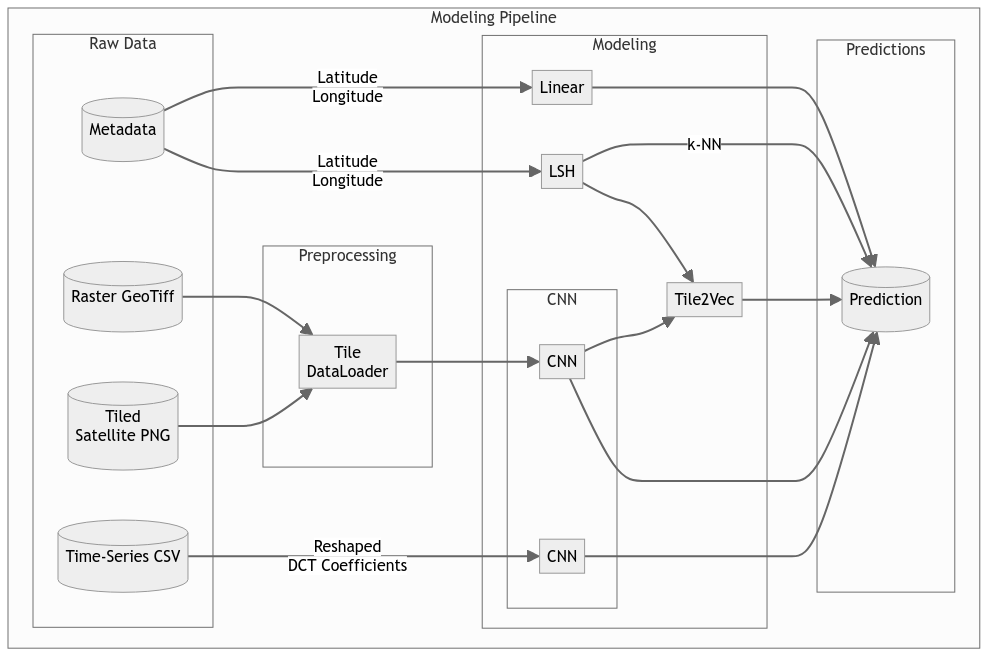
\includegraphics[width=\textwidth]{figures/pipeline4.png}
  \caption{
    Overview of the data and modeling pipeline.
    Raw data is pre-processed to maintain survey site per row semantics, with 2D DCT coefficients as features.
    Data is cached as columnar parquet files in cloud storage for efficient access.
  }
  \label{fig:tiled-raster}
\end{figure}

We explore several solutions for the multi-label classification problem. 
We use Luigi \cite{Rouhani2024spotify} as our workflow management tool, which provides idempotent directed acyclic graphs (DAGs) of tasks. 
We use Spark \cite{armbrust2015spark} to perform data extraction, transformation, and loading (ETL) from tarred images and CSV files to columnar parquet files. 
We use PyTorch as our deep learning framework and use PyTorch-Lightning to simplify the training and inference process.
We use Petastorm to preprocess and load data into Torch.
We use Weights and Biases to log hyperparameters and metrics.

\subsection{Satellite and Raster Data}

\begin{figure}[h!]
  \centering
  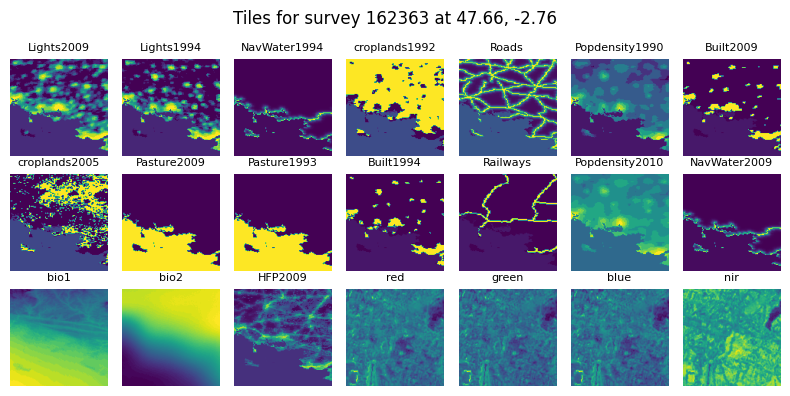
\includegraphics[width=\textwidth]{figures/tiles3.png}
  \caption{
      Example of a tiled raster image. 
      The image is a 128x128 tile of the RGB-NIR satellite imagery. 
      The image is associated with a survey site and is used as input to the model. 
  }
  \label{fig:tiled-raster}
\end{figure}

The competition organizers provide point data for each survey site in a pre-computed train CSV file.
Our experiments focus on 128x128 pixel tiles extracted from provided GeoTIFF files for use in a supervised learning setting.
Significant in-memory overhead tiling exists because we need to store a 128x128 matrix of integers or floats for each survey site.
Memory access patterns can cause significant slow-downs if we need to fetch them from disks often. 

We fork the official \texttt{plantnet/GeoLifeCLEF} data loaders to pre-compute tiles for each of the provided GeoTIFF under 1GB. 
Certain rasters do not fit into memory (e.g., elevation raster at 11GB); therefore, we omit them from our experiments. 
We only compute the tiles associated with the survey identifiers in our metadata, which helps limit the size of the resulting dataset. 

\subsection{Tile Compression via Discrete Cosine Transform (DCT)}

% three images side by side
\begin{figure}[h!]
  \centering
  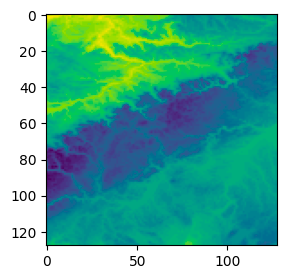
\includegraphics[width=0.3\textwidth]{figures/dct-original.png}
  \hfill
  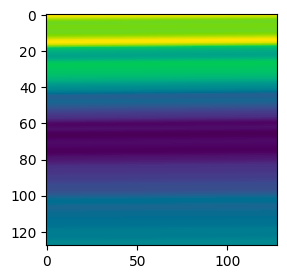
\includegraphics[width=0.3\textwidth]{figures/dct-1d-lowpass.png}
  \hfill
  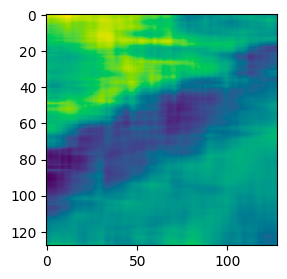
\includegraphics[width=0.3\textwidth]{figures/dct-2d-lowpass.png}
  \caption{
    Example of low-pass filtering using the DCT.
    (a) Original bio1 raster image.
    (b) Low-pass filter using the first 50 coefficients of the 1D-DCT, reshaping on the first axis (row-major order).
    (c) Low-pass filter using the 2D-DCT using the top-left 8x8 coefficients.
  }
  \label{fig:dct-lowpass}
\end{figure}

We computed the 2D-DCT on the resulting tile images and kept low-frequency coefficients as features in downstream modeling. 
We implement a PySpark wrapper around the ND-DCT to supplement the standard library 1D-DCT implementation for feature pre-processing.
We lose significant spatial information if we perform filtering in 1D coefficient-space as seen in Figure \ref{fig:dct-lowpass}.

\subsection{Time-Series Data}

Time series data are treated as another layer in the network by pre-processing the data to obtain DCT coefficients.
We have access to quarterly time series data for each survey site over 20 years.
Some sites have missing data, which are padded with zeros.
We compute the 1D DCT on the time series data and keep the first 64 coefficients in the transformed space, which parallels the 8x8 2D-DCT coefficients extracted from the raster data.
The original time-series data and its DCT are displayed side by side in figure \ref{fig:dct-timeseries}

% two images side by side
\begin{figure}[h!]
  \centering
  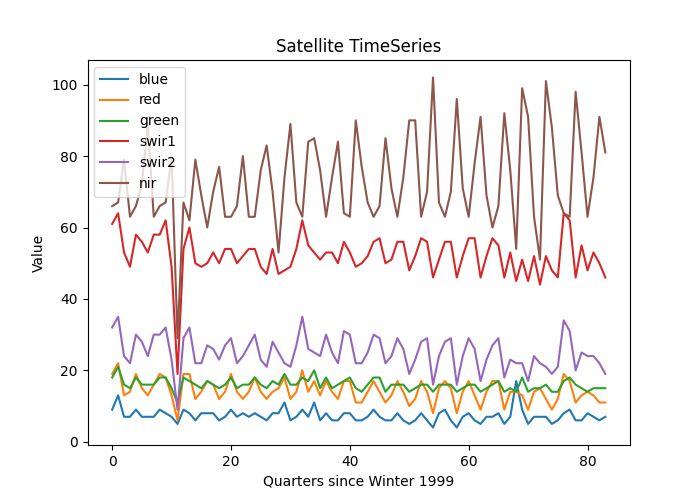
\includegraphics[width=0.495\textwidth]{figures/6-bands.png}
  \hfill
  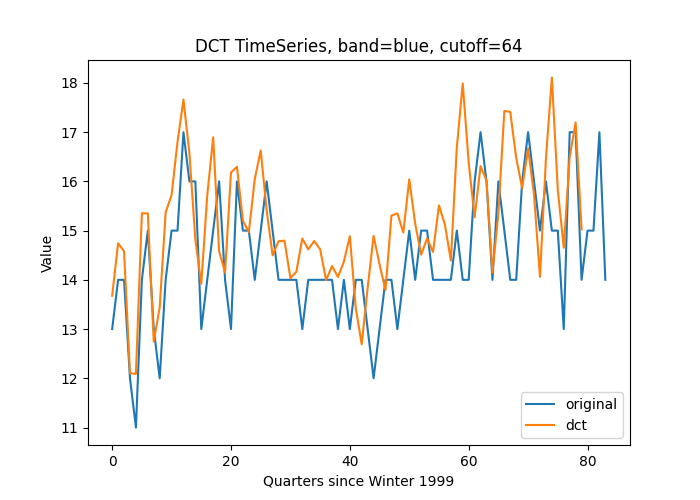
\includegraphics[width=0.495\textwidth]{figures/both.png}
  \caption{
    Example of time-series data and its DCT.
    (a) Original time-series data.
    (b) Blue band time-series approximated using DCT.
  }
  \label{fig:dct-timeseries}
\end{figure}

\subsection{Data Augmentation}

\begin{figure}[h!]
\begin{lstlisting}[language=Python,frame=single]
class DCTHorizontalFlip:
    def __init__(self, k=8):
        self.odd_factor = -torch.ones((k, k))
        for i in range(0, k, 2):
            self.odd_factor[i, :] = 1

    def forward(self, X):
        return X * self.odd_factor
\end{lstlisting}
\caption{Augmentation of 2D-DCT coefficients that flips the image across the horizontal axis in the spatial domain.}
\label{lst:augmentation}
\end{figure}

We apply augmentations to our data to encourage model invariance to rotation and reflection.
Some such transforms include rotating and flipping images before sending them into a model.
Equivalent augmentations exist in the frequency space.
For example, a 90-degree rotation in pixel space is equivalent to the transpose of the 2D-DCT coefficients.
We can flip the image in pixel space by alternating the signs of the 2D-DCT coefficients along a given axis.
Rotations and flips along the axis give us enough flexibility to implement useful symmetries in the data to improve model generalization.

\subsection{Locality-Sensitive Hashing for Nearest Neighbor Queries}

Species at sites close together should intuitively have similar distributions of plants. 
The projected latitude and longitude have physical meaning via euclidean distance, so we can build a nearest-neighbor model and rank species per survey site by frequency in a neighborhood.
We use locality-sensitive hashing (LSH) with random hyperplane projections to build a k-NN model \cite{leskovec2020mining}, with the hyper-parameters for bucket length and number of hash tables set to 20 and 5, respectively.
We can find the top-k nearest survey sites in linear time for any given survey site using the LSH model.
The approximate nearest neighbor self-join is performed with a 50km cutoff, and the results stored on disk for downstream modeling.
% We can construct several potential networks from our LSH representation: survey-survey, survey-species, and species-species. 
% We consider the species-species multi-network using a threshold of 100km quantized into 10km buckets and see that the majority of edges fall within the first 10km at 318M edges.

